\documentclass[border=10pt]{standalone}
\usepackage{amsmath,amssymb}
\usepackage{pgfplots}
\pgfplotsset{compat=1.18}
\usetikzlibrary{arrows.meta}
\usepackage{amsmath}

\begin{document}
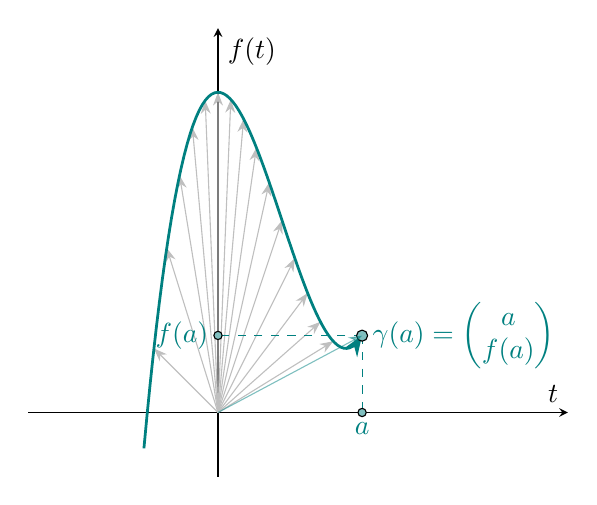
\begin{tikzpicture}
% --- Pre-calculate all values for the new function ---
\pgfmathsetmacro{\a}{2.25}              % x-coordinate of point p
\pgfmathsetmacro{\ay}{\a^3-3*\a^2+5} % y-coordinate using the new function
\pgfmathsetmacro{\slope}{3*\a^2 -6*\a} % Slope using the new derivative

\pgfmathsetmacro{\dx}{1}             % Vector x-component (made slightly smaller for visibility)
\pgfmathsetmacro{\dy}{\slope * \dx}   % Vector y-component
\pgfmathsetmacro{\endx}{\a + \dx}     % Vector end-point x
\pgfmathsetmacro{\endy}{\ay + \dy}     % Vector end-point y

% --- Pre-calculate label position for the tangent line ---
\pgfmathsetmacro{\labelx}{\a + 0.5}
\pgfmathsetmacro{\labely}{\ay + \slope*(\labelx-\a)}

\begin{axis}[
axis lines=center,
xlabel=$t$,xtick=\empty,
ylabel=$f(t)$,ytick=\empty,
legend pos=north west,
xmin=-2.5, xmax=5,   % Adjusted axis limits
ymin=-1, ymax=6,    % Adjusted axis limits
restrict y to domain=-1:6,
axis equal, % Ensures slopes are visually correct
clip=false,
]
\pgfplotsextra{
	\foreach \a in {-1, -.8, ..., 1.8} {
		\pgfmathsetmacro{\dx}{1}
		
		% Compute f(a) = a^3 - 3a^2 + 5
		\pgfmathparse{\a*\a*\a - 3*\a*\a + 5}
		\edef\ay{\pgfmathresult}
		
		% Draw arrow
		\edef\cmd{
			\noexpand\draw[-{Stealth}, gray!50]
			(axis cs:0,0) -- (axis cs:\a,\ay); 
			%			node[right] {$\langle 1, f'(\a)\rangle$};
		}
		\cmd
	}
}

% --- Mark the point p ---
%	\node[circle, fill=magenta, inner sep=1.5pt, label={above:$\color{magenta}p$}] at (axis cs: \a, \ay) {};
\draw[dashed, teal] (\a,\ay) to (\a,0) node[below] {$a$};
\draw[dashed, teal] (\a,\ay) to (0,\ay) node[left] {$f(a)$};

\addplot[-{Stealth}, domain=-2.5:2.25, samples=100, line width=.35mm, teal] {(x+1)*(x-2)*(x-2) + 1} node[right] {$\gamma(a)=\begin{pmatrix}
		a \\ f(a)
	\end{pmatrix}$};
\draw[fill=teal!50] (2.25,1.2) circle (2pt);
\draw[-{Stealth}, teal, opacity=.5] (0,0) to (2.25,1.2);
\draw[fill=teal!50] (\a,0) circle (1.5pt);
\draw[fill=teal!50] (0,\ay) circle (1.5pt);
\end{axis}
\end{tikzpicture}
\end{document}